\documentclass[11pt]{article}
\usepackage[margin=0.7in]{geometry}
\usepackage{booktabs}
\usepackage{tikz}
\usetikzlibrary{shapes.geometric, arrows.meta, positioning, calc, fit, backgrounds}
\usepackage{hyperref}

% ---------------------------------------------------------------------------
% PRISMA flow diagram styles. Prototype -- tweak sizes/colours freely.
% ---------------------------------------------------------------------------
\definecolor{spine}{HTML}{1F5E66}
\definecolor{drop}{HTML}{A03E28}
\definecolor{hold}{HTML}{8A6520}
\definecolor{rule}{HTML}{B8C2C7}
\definecolor{bandbg}{HTML}{EEF2F3}

\tikzset{
  box/.style   = {draw=rule, line width=0.5pt, fill=white, text width=#1,
                  align=left, inner sep=6pt, font=\footnotesize,
                  minimum height=1.05cm, rounded corners=1pt},
  main/.style  = {box=6.6cm, draw=spine, line width=1pt},
  out/.style   = {box=6.4cm, draw=drop, densely dashed},
  held/.style  = {box=6.4cm, draw=hold, densely dashed},
  flow/.style  = {-{Latex[length=2.2mm,width=1.6mm]}, draw=spine, line width=0.9pt},
  side/.style  = {-{Latex[length=2.2mm,width=1.6mm]}, draw=drop, line width=0.7pt},
  phase/.style = {rotate=90, font=\bfseries\scriptsize, text=spine,
                  anchor=center, align=center},
}

\title{Corpus Disposition: PRISMA Flow}
\author{Cluster-Paper Review}
\date{\today}

\begin{document}
\maketitle
\vspace{-2em}

\noindent
Companion to \texttt{results/corpus\_disposition.tex}, which carries the same numbers as tables.
Two sets are tracked separately: the \textbf{Unlabelled Set} (to be classified by the model) and the
\textbf{Human Labelled Set} (already reviewed by NCI or NHLBI). Solid boxes are the main flow; dashed
red boxes are papers leaving; dashed amber boxes are papers held pending a human decision.

\vfill

\section*{Unlabelled Set}

\begin{center}
\begin{tikzpicture}[node distance=8mm]

\node[main] (a1) {\textbf{2115} raw Zotero items\\[1pt]\scriptsize 23 institute subcollections under \emph{Boring Task}};
\node[main, below=of a1] (a2) {\textbf{1494} unique papers\\[1pt]\scriptsize All fetched, md5-checked, zero failures};
\node[main, below=of a2] (a3) {\textbf{1287} papers not already labelled};
\node[main, below=of a3] (a4) {\textbf{1284} active Unlabelled Set\\[1pt]\scriptsize Full text extracted and cached};

\node[out, right=14mm of $(a1)!0.5!(a2)$] (x1)
  {$-621$ collapsed or skipped\\[1pt]\scriptsize 619 multi-institute placements (483 papers filed 2--6 times); 2 non-article items};
\node[out, right=14mm of $(a2)!0.5!(a3)$] (x2)
  {$-207$ cross-set duplicates\\[1pt]\scriptsize Already in the Labelled Set, where the paper carries a human answer};
\node[out, right=14mm of $(a3)!0.5!(a4)$] (x3)
  {$-3$ correction notices\\[1pt]\scriptsize An erratum is not a study. Dropped by hand, files preserved};

\draw[flow] (a1) -- (a2);
\draw[flow] (a2) -- (a3);
\draw[flow] (a3) -- (a4);
\draw[side] ($(a1)!0.5!(a2)$) -- (x1);
\draw[side] ($(a2)!0.5!(a3)$) -- (x2);
\draw[side] ($(a3)!0.5!(a4)$) -- (x3);

\end{tikzpicture}
\end{center}

\noindent\footnotesize
The collection \texttt{sample NCI-new} (104 papers) was excluded before this diagram begins and never
fetched. Seven further papers are owed back into this set --- see \emph{Papers now in neither set} below.

\newpage
\section*{Human Labelled Set}

\begin{center}
\begin{tikzpicture}[node distance=8mm]

\node[main] (b1) {\textbf{569} fetched from two Zotero groups\\[1pt]\scriptsize NCI 232 + NHLBI 337. All passed identity verification};
\node[main, below=of b1] (b2) {\textbf{554} manifest rows};
\node[main, below=of b2] (b3) {\textbf{553} after correction notice};
\node[main, below=of b3] (b4) {\textbf{530} active Human Labelled Set};
\node[main, below=of b4] (b5) {\textbf{523} loaded into the label table};
\node[main, below=of b5] (b6) {\textbf{492} scoreable for exclusion\\[1pt]\scriptsize 316 exclude / 176 keep};
\node[main, below=of b6] (b7) {\textbf{176} pass the gate\\[1pt]\scriptsize Carry power and data-analysis labels};

\node[out, right=14mm of $(b1)!0.5!(b2)$] (y1)
  {$-15$ internal duplicates merged\\[1pt]\scriptsize Same paper in both groups under different item keys; NCI key kept, 9 of 15 byte-identical};
\node[out, right=14mm of $(b2)!0.5!(b3)$] (y2)
  {$-1$ correction notice\\[1pt]\scriptsize \texttt{JBUFJCLU}};
\node[out, right=14mm of $(b3)!0.5!(b4)$] (y3)
  {$-23$ cited but never reviewed\\[1pt]\scriptsize Blank in every label column; the NHLBI review will not resume};
\node[held, right=14mm of $(b4)!0.5!(b5)$] (y4)
  {$-7$ held for adjudication\\[1pt]\scriptsize 6 institutional disagreements (only 3 genuine) + 1 unresolved citation};
\node[out, right=14mm of $(b5)!0.5!(b6)$] (y5)
  {$-31$ random tie-break exclusions\\[1pt]\scriptsize A coin flip over which other papers share a first author --- not learnable from one PDF};
\node[held, right=14mm of $(b6)!0.5!(b7)$] (y6)
  {$-316$ excluded by the reviewers\\[1pt]\scriptsize No power or data-analysis label exists for these, by design};

\draw[flow] (b1) -- (b2);
\draw[flow] (b2) -- (b3);
\draw[flow] (b3) -- (b4);
\draw[flow] (b4) -- (b5);
\draw[flow] (b5) -- (b6);
\draw[flow] (b6) -- (b7);
\draw[side] ($(b1)!0.5!(b2)$) -- (y1);
\draw[side] ($(b2)!0.5!(b3)$) -- (y2);
\draw[side] ($(b3)!0.5!(b4)$) -- (y3);
\draw[side, draw=hold] ($(b4)!0.5!(b5)$) -- (y4);
\draw[side] ($(b5)!0.5!(b6)$) -- (y5);
\draw[side, draw=hold] ($(b6)!0.5!(b7)$) -- (y6);

\end{tikzpicture}
\end{center}

\newpage
\section*{Papers now in neither set}

An edge case created by ordering: the cross-set duplicate check ran before the Labelled Set was final.
Twelve of the 207 papers removed from the Unlabelled Set have since lost their labelled copy.

\begin{center}
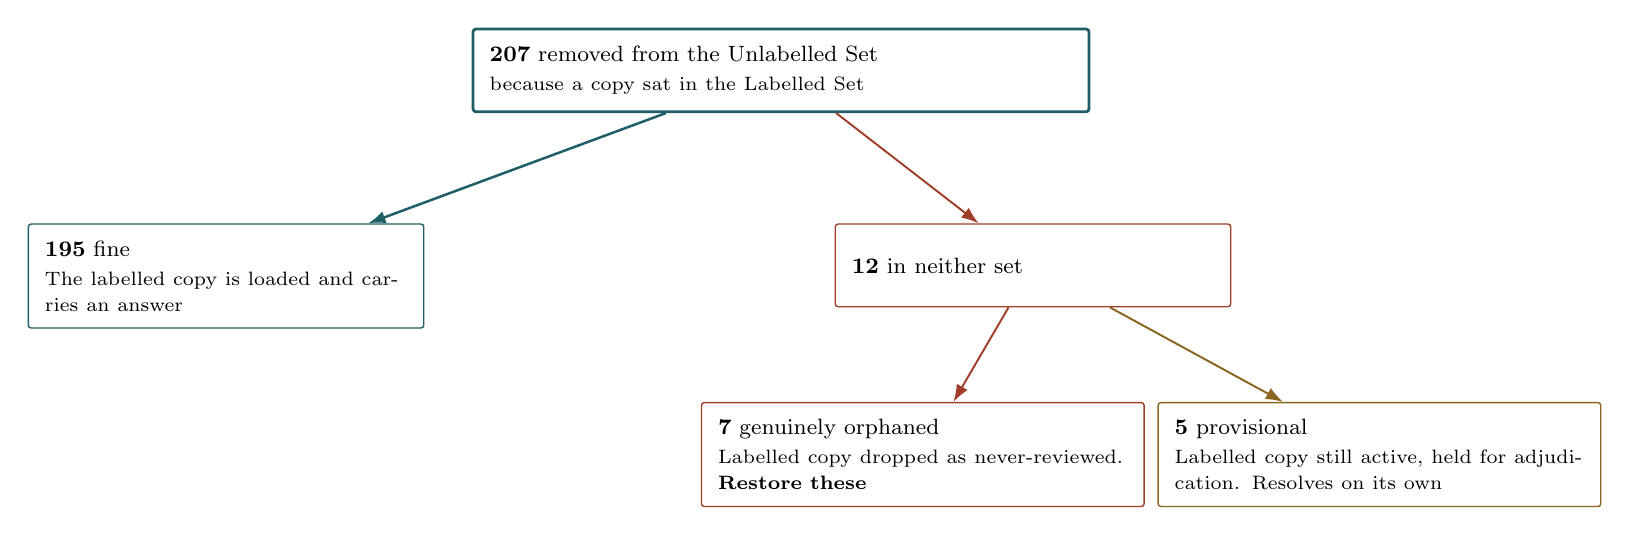
\begin{tikzpicture}[node distance=9mm]

\node[main, text width=7.4cm] (c1)
  {\textbf{207} removed from the Unlabelled Set\\[1pt]\scriptsize because a copy sat in the Labelled Set};
\node[box=4.6cm, draw=spine, below left=14mm and 6mm of c1] (c2)
  {\textbf{195} fine\\[1pt]\scriptsize The labelled copy is loaded and carries an answer};
\node[box=4.6cm, draw=drop, below=14mm of c1, xshift=32mm] (c3)
  {\textbf{12} in neither set};
\node[box=5.2cm, draw=drop, below=12mm of c3, xshift=-14mm] (c4)
  {\textbf{7} genuinely orphaned\\[1pt]\scriptsize Labelled copy dropped as never-reviewed. \textbf{Restore these}};
\node[box=5.2cm, draw=hold, below=12mm of c3, xshift=44mm] (c5)
  {\textbf{5} provisional\\[1pt]\scriptsize Labelled copy still active, held for adjudication. Resolves on its own};

\draw[flow] (c1) -- (c2);
\draw[side] (c1) -- (c3);
\draw[side] (c3) -- (c4);
\draw[side, draw=hold] (c3) -- (c5);

\end{tikzpicture}
\end{center}

\noindent
The seven to restore: \texttt{EMQMPLJ5}, \texttt{DH6IG7JY}, \texttt{N35XJ5YV}, \texttt{4GPSLLBZ},
\texttt{FP3HZHGS}, \texttt{TCS56FZY}, \texttt{VH6KS89D}. PDFs and cached text were never deleted, so
restoring is a manifest edit rather than a refetch. Re-run this check after any future change to the
Labelled Set --- the edge case recurs every time a labelled paper is dropped.

\section*{What the model will be scored on}

\begin{table}[h]
\centering
\begin{tabular}{lrrr}
\toprule
\textbf{Task} & \textbf{Papers} & \textbf{Class split} & \textbf{Majority baseline} \\
\midrule
Exclusion      & 492 & 316 exclude / 176 keep     & 64\% \\
Power analysis & 176 & 136 incorrect / 40 correct & 77\% \\
Data analysis  & 176 & 129 incorrect / 47 correct & 73\% \\
\bottomrule
\end{tabular}
\end{table}

\noindent
All three tasks are imbalanced, so plain accuracy is not a meaningful headline: a model answering
``incorrect'' to every power analysis scores 77\% while learning nothing. Report balanced accuracy,
macro-F1, and Cohen's $\kappa$, each beside its majority-class baseline, with the full confusion
matrix. Because this compares a model to human reviewers rather than to objective truth --- the source
paper describes its own labels as ``the opinion of two knowledgeable reviewers \dots\ rather than an
objective classification scheme'' --- $\kappa$ is the appropriate statistic, and the 80\% NCI--NHLBI
agreement rate is the ceiling to read it against.

\end{document}
